\cotefile{123}
\scanpage{2}
Compléments sur transformation de Coxeter d'un système de racines\inserted{\handwritten{\unsure{irréductible|irreductible}}} (Kostant).
\margin{\handwritten{The principal 3-dimensional subgroup ....\quad th. 9.2.}}
% The inserted word is above the title in an oval, with a leader to before ``(Kostant)''.
\margin{\handwritten{\figure{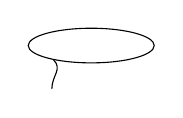
\begin{tikzpicture}[x=1cm,y=1cm]\draw (0,0) ellipse (0.8 and 0.22);\draw (-0.48,-0.18) .. controls (-0.36,-0.3) and (-0.5,-0.38) .. (-0.5,-0.55);\end{tikzpicture}}}}

a) Soit $w\handwritten{\in}W$. Alors toute valeur propre de $w$ \unsure{est} une racine de $1$ d'ordre divisant un des entiers $m_i+1$ (où les $m_i$ sont les exposants caractéristiques), donc d'ordre $\handwritten{\leq}h$. Pour qu'il y en ait une qui soit d'ordre $h$, il faut et suffit que $w$ soit une transformation de Coxeter, et\inserted{alors} les éléments non nuls du sous-espace propre correspondant\handwritten{\raisebox{-0.5ex}{$\circ$}} sont des éléments réguliers.
% Left marginal insertion; its words ascend at different angles rather than forming two straight lines.
\margin{\inserted{\handwritten{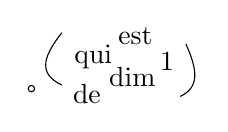
\begin{tikzpicture}[x=0.9cm,y=0.9cm,baseline=(qui.base)]
\node[anchor=base west,inner sep=0] (qui) at (0,0.05) {qui};
\node[anchor=base west,inner sep=0] at (0.62,0.31) {est};
\node[anchor=base west,inner sep=0] at (-0.02,-0.52) {de};
\node[anchor=base west,inner sep=0] at (0.49,-0.28) {dim};
\node[anchor=base west,inner sep=0] at (1.21,-0.05) {1};
\draw (-0.17,0.48) .. controls (-0.47,0.10) and (-0.48,-0.11) .. (-0.17,-0.26);
\draw (1.58,0.32) .. controls (1.75,-0.06) and (1.77,-0.29) .. (1.50,-0.42);
\draw (-0.60,-0.31) circle (0.045);
\end{tikzpicture}}}}
\margin{\handwritten{\figure{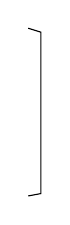
\begin{tikzpicture}[x=1cm,y=1cm]\draw (-0.16,0.05)--(0,0)--(0,-2.05)--(-0.16,-2.08);\end{tikzpicture}}}}

\uline{Corollaire}\handwritten{1}: Soit $\handwritten{\mu}$ le sous-groupe de $W$ engendré par un élément de Coxeter $c$, donc $\handwritten{\mu\simeq}\underline{Z}\handwritten{/}h\underline{Z}$. Alors $\handwritten{\mu}$ est égal au centralisateur de $c$, donc de $\handwritten{\mu}$, et si $\handwritten{\nu}$ est le normalisateur de $\handwritten{\mu}$, l'homomorphisme
\margin{\handwritten{\figure{\begin{tikzpicture}[x=1cm,y=1cm]\draw (0,0)--(0,-2.4);\end{tikzpicture}}}}
\[
\handwritten{\unsure{\psi|\nu}/\mu\longrightarrow}\operatorname{Aut}(\handwritten{\mu})\handwritten{\simeq}(\underline{Z}/h\underline{Z})^{\handwritten{*}}
\]
\margin{\handwritten{\shortstack[l]{Quelle extension\\de $(\unsure{Z|\mathbb{Z}}/hZ]^{*}$ par\\$\mathbb{Z}/h\mathbb{Z}$ \unsure{obtient-on} ?}}}
est \unsure{un} isomorphisme; en d'autres termes, pour tout entier $n$ premier à $h$, il existe un $w\handwritten{\in}W$ tel que $wcw^{-1}=c^h$, et $w$ est déterminé mod $\handwritten{\mu}$.
\margin{\handwritten{\unsure{échanger|échange} avec cor. 3}}
% slanted

Soit \unsure{en} ef\inserted{f}et $D$ \deleted{\unsure{une droite}}\inserted{le sous-espace} propre sous $c$ correspondant à une racine primitive $h$.ème de $1$. Alors $\dim D=1$ (prop.\handwritten{30}), et $\handwritten{\unsure{\mathfrak{z}|z}}=\operatorname{Centr}(\handwritten{\mu})$ normalise $D$, d'où un homomorphisme $\handwritten{\mathfrak{z}\to}\operatorname{Aut}(D)=\underline{C}^{\handwritten{*}}$, dont l'image est un sous-groupe fini de $\underline{C}^{\handwritten{*}}$, contenant l'image (isomorphe) de $\handwritten{\mu}$, donc cyclique d'ordre un multiple de $h$. Grâce à Kostant, son ordre est égal à $h$, et on a donc trouvé une rétraction $\handwritten{\mathfrak{z}\to\mu}$, il faut prouver que son noyau est réduit à $1$. Or si $w$ est dans ce noyau, il \deleted{induit} centralise $D$, et \unsure{qômme} $D$ est régulière par Kostant,cela implique $w=1$. \unsure{On|Bn} a donc prouvé $\handwritten{\mathfrak{z}}=\handwritten{\mu}$. Reste à prouver que si $n$ est un entier premier à $h$, alors $c^n$ est conjugué de $c$, ce qui résulte également de Kostant.

\uline{Corollaire}. Soit $c$ un élément de Coxeter, et $\handwritten{\lambda}$ une valeur propre de $c$, correspondant à un vecteur propre $x$. Pour que $x$ soit régulier, il faut et il suffit que $\handwritten{\lambda}$ soit une racine primitive $h$.ème de $1$.
\margin{\handwritten{\figure{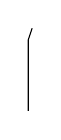
\begin{tikzpicture}[x=1cm,y=1cm]\draw (0.05,0)--(0,-0.15)--(0,-1.05);\end{tikzpicture}}}}

La suffisance a déjà été énoncée avec le th. de Kostant. Pour la nécessité, soit $h'\handwritten{\leq}h$ l'ordre de la valeur propre, alors $\unsure{\mathbin{.}}c^{h'}$ centralise $x$, donc, $x$ étant régulier, on a $c^{h'}=1$, donc $h'=h$, cqfd.

\uline{Corollaire}. \deleted{\unsure{Considérons}} \deleted{Soit $D$ une}\inserted{Soit $D$ une} droite régulières dans $V\unsure{\otimes|\mathbin{\text{\textcircled{x}}}}\underline{C}$ telle qu'il existe un élé%
% archive sheet number: 1
